% begin module volumes-otherline
\begin{frame}
\begin{example}[Rotated About a Line Other Than the $x$-axis]
Find the volume of the solid obtained by rotating about the line $y = 1$ \alert<handout:0| 4>{the region bounded by \alert<handout:0| 2>{$y = -x^2+2x+1$} and \alert<handout:0| 3>{$y = 1$}.}

\uncover<5->{%
The typical cross-section is a circle centered at $(x, 1)$.
}%

\uncover<6->{%
\alert<handout:0| 6-7>{Area of cross-section: \uncover<7->{$\pi ((-x^2+2x+1)-1)^2$}}
}%
\begin{columns}[c]
\column{.4\textwidth}
\begin{center}
\only<handout:0| 1>{%
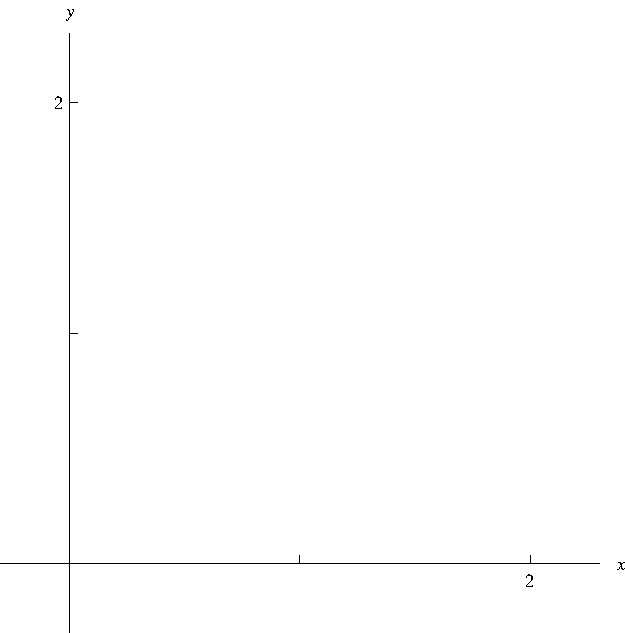
\includegraphics[height=5cm]{volumes/pictures/06-02-otherlinea.pdf} %
}%
\only<handout:0| 2>{%
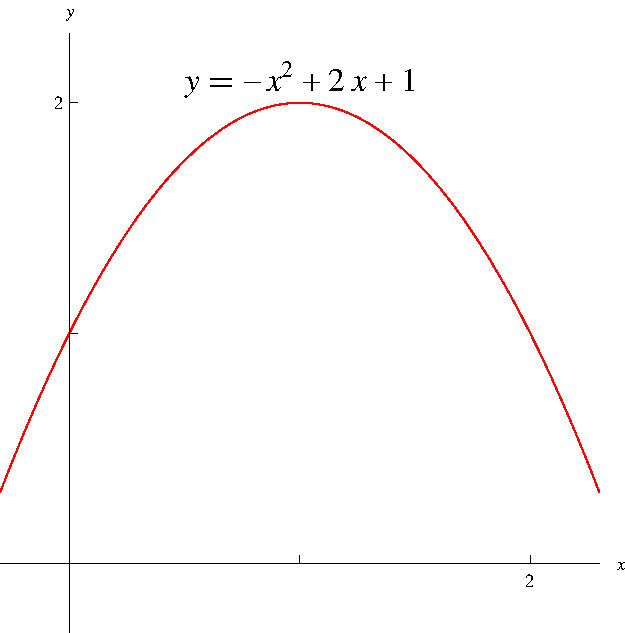
\includegraphics[height=5cm]{volumes/pictures/06-02-otherlineb.pdf} %
}%
\only<handout:0| 3>{%
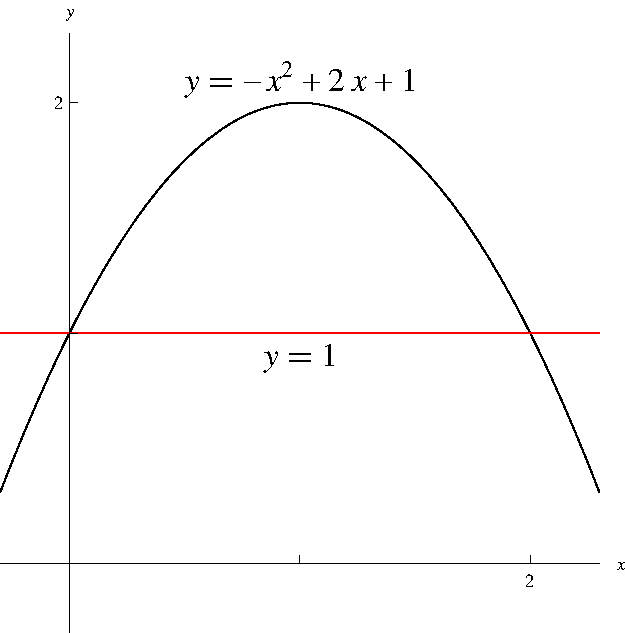
\includegraphics[height=5cm]{volumes/pictures/06-02-otherlinec.pdf} %
}%
\only<handout:0| 4>{%
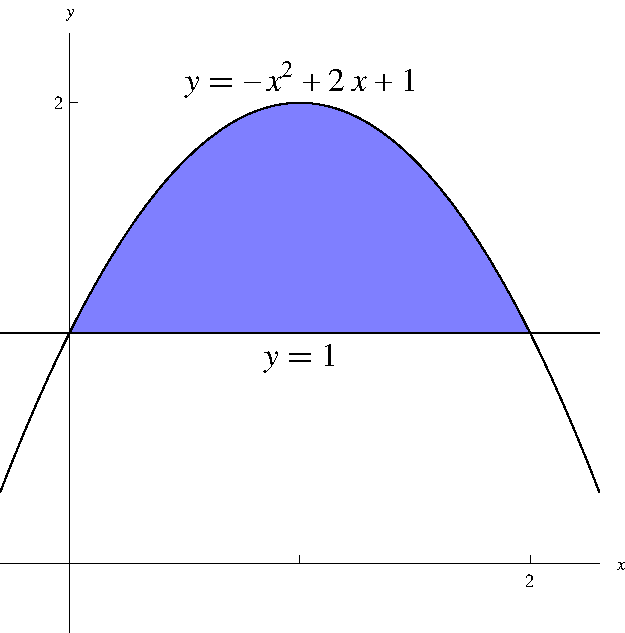
\includegraphics[height=5cm]{volumes/pictures/06-02-otherlined.pdf} %
}%
\only<5->{%
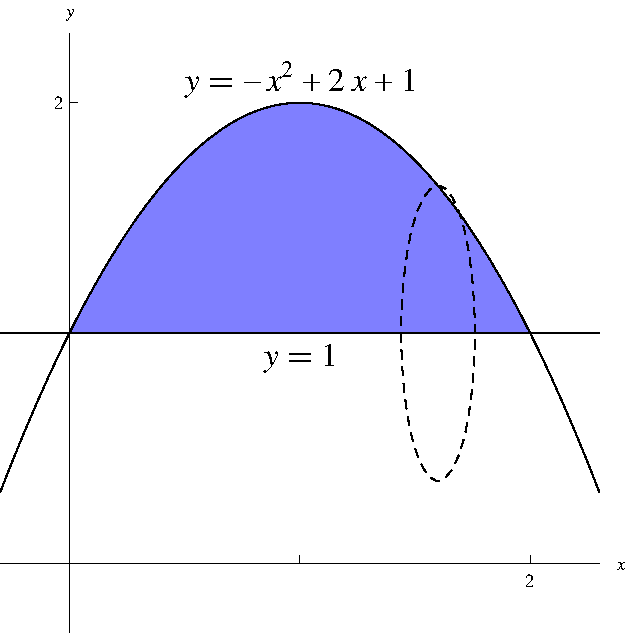
\includegraphics[height=5cm]{volumes/pictures/06-02-otherlinee.pdf} %
}%
\end{center}
\column{.6\textwidth}

\abovedisplayskip=0pt
\belowdisplayskip=0pt
\abovedisplayshortskip=0pt
\belowdisplayshortskip=0pt
\begin{align*}
\uncover<8->{%
V%
}%
& \uncover<8->{ = } %
\uncover<8->{%
\int_0^2  \pi \left( (-x^2+2x+1) -  1\right)^2  \ \diff x%
}\\%
& \uncover<9->{ = } %
\uncover<9->{%
\pi \int_0^2 \left( \alert<handout:0| 10-11>{x^4} - \alert<handout:0| 12-13>{4x^3} + \alert<handout:0| 14-15>{4x^2} \right) \  \diff x%
}\\%
& \uncover<10->{ = } %
\uncover<10->{%
\pi \left[ \alert<handout:0| 11>{\uncover<11->{\frac{x^5}{5}}} - \alert<handout:0| 13>{\uncover<13->{x^4}} + \alert<handout:0| 15>{\uncover<15->{\frac{4x^3}{3}}} \right]_0^2%
}\\%
& \uncover<16->{ = } %
\uncover<16->{%
\pi \left( \frac{32}{5} - 16 + \frac{32}{3} \right) \uncover<17->{= \frac{16}{15}\pi}
}%
\end{align*}
\end{columns}
\end{example}
\end{frame}
% end module volumes-otherline
